% background chapter continued
\section{Mercator Architecture}\label{blueprint}
This section proceeds into detailed description of Mercator web crawler surveyed in section \ref{relatedworks}. Figure \ref{fig:basicarch} is a high-level composition of the same. As seen, Mercator specializes different steps defined in basic crawling
algorithm covered in section \ref{basicalgo} and adds several other steps to address
the social and scalability challenges of web crawler. Its blueprint design offers
horizontal scalability and therefore if implemented can run on more than one node.
Each part that contributes to mercator crawler can also be referred to as a
component, module, subsystem, etc. They can be used interchangeably from this point onward.

\begin{figure}[h!]
  \centering
  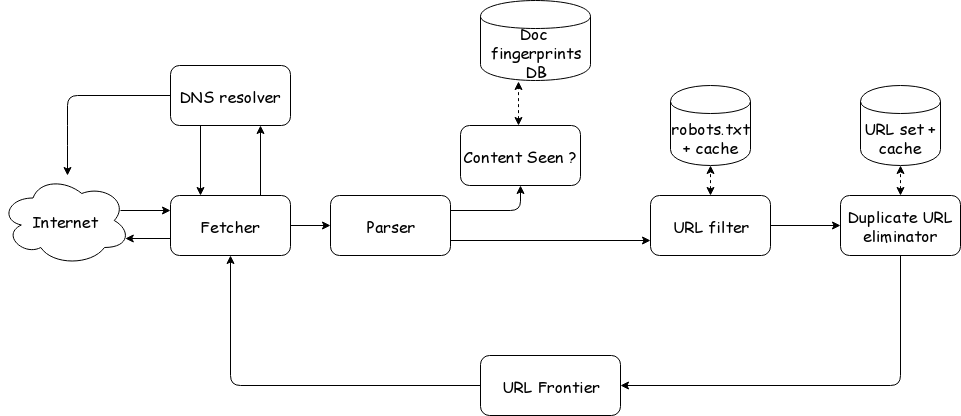
\includegraphics[width=15cm,height=12cm,keepaspectratio]{../media/crawler/basic-crawler-architecture-v2.png}
  \caption{High-level organization of Mercator}
  \label{fig:basicarch}
\end{figure}

\noindent
Each work cycle begins and ends at the URL Frontier. Depending on what needs to be
achieved, the entire crawler can run as a single process or can be partitioned into multiple processes - treating each subsystem as a process. Given a single URL, it
goes through the cycle of being fetched followed by passing through various checks,
filters and eliminations, then finally returned to the Frontier (for incremental crawling).
\\
\\
At the beginning of each logical loop cycle, a worker thread pops a URL from the Frontier data structure adhering to the priority and politeness policy. The output URL is then fetched by HTTP fetcher subsystem - which like any other web client contacts DNS module to get IP address of the corresponding web server. The web page is then retrieved and stored at a temporary location which is then picked up by parser subsystem which forwards extracted text and extracted links to content seen and URL filter, respectively. The batch of URLs undergo a fixed set of pre-processing steps at the URL filter subsystem before being passed over to Duplicate URL eliminator (DUE). The DUE module tests each URL to determine whether the link should be added to the
URL frontier.


\subsection{Fetcher, Parser, and DNS}\index{Fetcher, Parser, and DNS}
\subsection{Handling De-duplication}\index{Handling De-duplication}
\subsection{URL Filtering}\index{URL Filtering}
\subsection{Duplicate URL Eliminator (DUE)}\index{Duplicate URL Eliminator(DUE)}

\pagebreak

\subsection{URL Frontier}
some text here
\begin{figure}[h!]
  \centering
  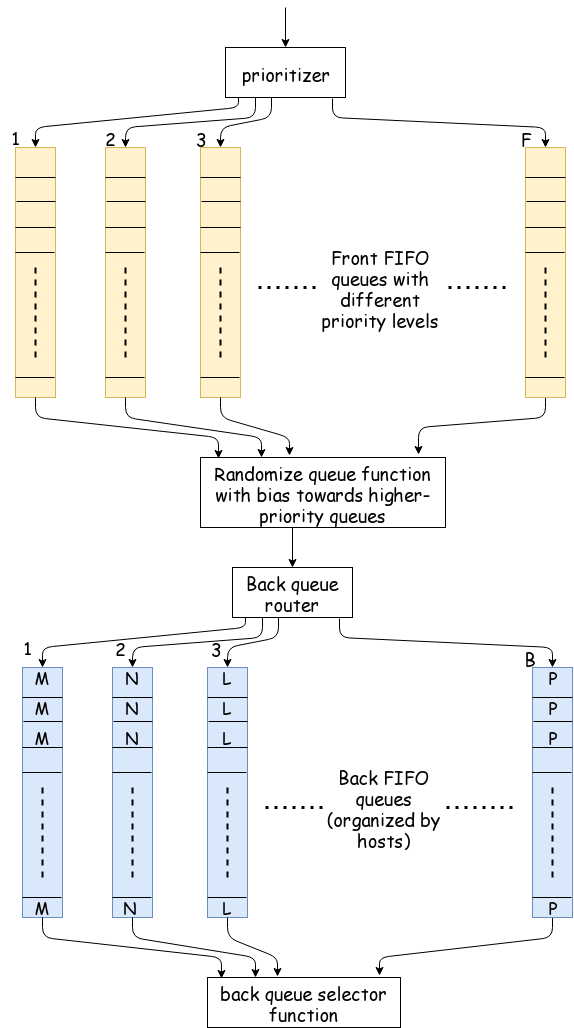
\includegraphics[width=10cm,height=13cm,keepaspectratio]{../media/crawler/url-frontier.png}
  \caption{URL Frontier Scheme(based on Mercator)}
  \label{fig:frontier}
\end{figure}

\pagebreak
some text here
\begin{figure}[h!]
  \centering
  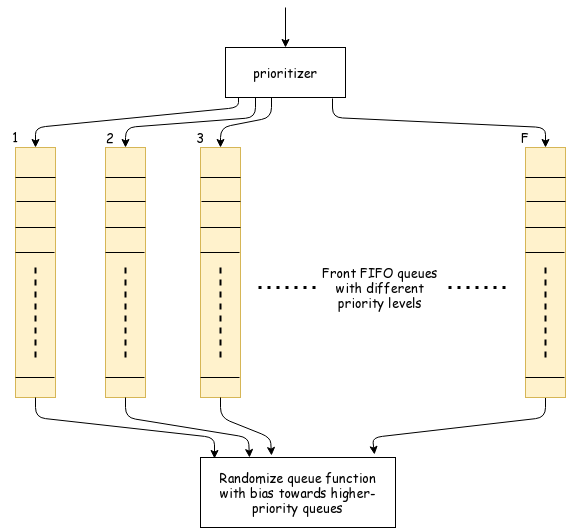
\includegraphics[width=13cm,height=10cm,keepaspectratio]{../media/crawler/f-queue.png}
  \caption{Frontier Front Queue}
  \label{fig:fqueue}
\end{figure}

\pagebreak
some text here
\begin{figure}[h!]
  \centering
  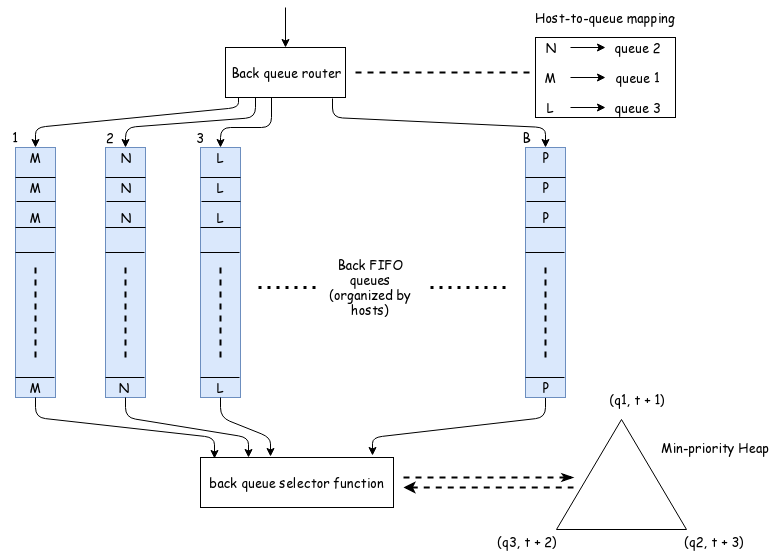
\includegraphics[width=13cm,height=10cm,keepaspectratio]{../media/crawler/b-queue.png}
  \caption{Frontier Back Queue}
  \label{fig:bqueue}
\end{figure}

\pagebreak
some text here
\subsection{Distributing Web Crawl}\index{Distributing Web Crawl}
\begin{figure}[h!]
  \centering
  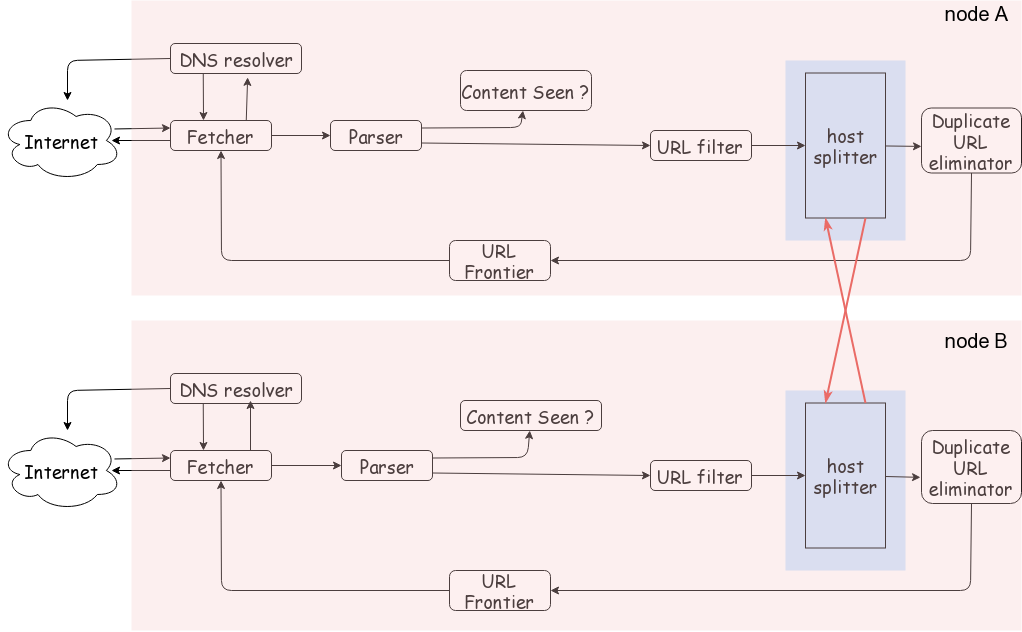
\includegraphics[width=15cm,height=10cm,keepaspectratio]{../media/crawler/host-splitterv3.png}
  \caption{Host Partitioning}
  \label{fig:hpart}
\end{figure}

\pagebreak

\section{Automata Analogy}\index{Automata Analogy}